\documentclass[dvipdfmx]{jsarticle}
\usepackage[top=1cm,bottom=1.0cm,left=1.0cm,right=1.0cm]{geometry}
\usepackage{listings,jlisting}
\usepackage{mips}
\usepackage{amssymb} % needed for math
\usepackage{amsmath} % needed for math
\usepackage[utf8]{inputenc} % this is needed for german umlauts
\usepackage[ngerman]{babel} % this is needed for german umlauts
\usepackage[T1]{fontenc}    % this is needed for correct output of umlauts in pdf
% the following is needed for syntax highlighting
\usepackage[dvipdfmx]{color}
\usepackage{tikz}
\usepackage{graphicx}
\usepackage{url}
\usepackage{nonfloat}

\usetikzlibrary{positioning}
\usetikzlibrary{shapes.callouts}



\definecolor{dkgreen}{rgb}{0,0.6,0}
\definecolor{gray}{rgb}{0.5,0.5,0.5}
\definecolor{mauve}{rgb}{0.58,0,0.82}

\lstset{ %
  language=C,       % the language of the code
  basicstyle=\ttfamily,       % the size of the fonts that are used for the code
  numbers=left,                   % where to put the line-numbers
  numberstyle=\color{gray},  % the style that is used for the line-numbers
  stepnumber=1,                   % the step between two line-numbers. If it's 1, each line
                                  % will be numbered
  numbersep=5pt,                  % how far the line-numbers are from the code
  backgroundcolor=\color{white},  % choose the background color. You must add \usepackage{color}
  showspaces=false,               % show spaces adding particular underscores
  showstringspaces=false,         % underline spaces within strings
  showtabs=false,                 % show tabs within strings adding particular underscores
  frame=single,                   % adds a frame around the code
  rulecolor=\color{black},        % if not set, the frame-color may be changed on line-breaks within not-black text (e.g. commens (green here))
  tabsize=4,                      % sets default tabsize to 2 spaces
  breaklines=true,                % sets automatic line breaking
  breakatwhitespace=false,        % sets if automatic breaks should only happen at whitespace
  title=\lstname,                 % show the filename of files included with \lstinputlisting;
                                  % also try caption instead of title
  keywordstyle=\color{blue},          % keyword style
  commentstyle=\color{dkgreen},       % comment style
  stringstyle=\color{mauve},         % string literal style
  escapeinside={\%*}{*)},            % if you want to add a comment within your code
  morekeywords={*,...},              % if you want to add more keywords to the set
  xleftmargin=17pt,
  framexleftmargin=17pt
}

\title {チーム開発におけるgitの使用手順}
\author{池守和槻 \and 著者名2}
\date{2009/05/24}
\begin{document}

  % タイトル出力
  \maketitle
  \section{はじめに}
    今回の開発では「Shared Repository Model」に基づいた開発をするための手順書である。\\
    「Shared Repository Model」を以下では「SRM」と略して書く。\\


  \section{SRMとは}
    SRMとは複数の開発者(少人数であることが多い)が1つのRepositoryのpush機能を保持し、Forkをせずに開発するモデルである。
    詳しくは、以下のサイトを参照 \\
    \url{https://help.github.com/en/articles/about-collaborative-development-models}

  \section{SRMによる開発の流れ}
    \begin{enumerate}
      \item 開発するRepositoryを自分のマシンのローカルにcloneする。
      \item master branchから開発用branchを作成
      \item 開発用branchで開発作業を行う
      \item 開発中のcommitは開発用のbranchにcommitする。
      \item 開発が終了したら、remote repositoryの開発用branchにpushしpull requestをする。
      \item コードレビューをして問題がなかったら、masterにmergeする。
    \end{enumerate}

    \subsection{具体例}
      $\\ \\$
      \begin{tikzpicture}[every node/.style={circle,fill=cyan,white}]
          \node (m0) {master};
          \node[right=of m0] (m1) {};
          \node[right=6.5cm of m1] (m2) {merge};
          \node[right=of m2] (m3) {};
          \node[below right=of m1] (d0) {develop};
          \node[right=of d0] (d1) {};
          \node[right=of d1] (d2) {};
          \node[right=of d2] (d3) {};

          \foreach \u / \v in {m0/m1,m1/m2,m2/m3,m1/d0,d0/d1,d1/d2,d2/d3,d3/m2}
            \draw[-] (\u) -- (\v);
      \end{tikzpicture}
      $\\ \\$
    以上のような開発フローを考える
    \begin{enumerate}
      \item 開発するRepositoryを自分のマシンのローカルにcloneする。
      \item masterブランチから開発ブランチを作成\\
        \begin{tikzpicture}[every node/.style={circle,fill=cyan,white}]
            \node (m0) {master};
            \node[right=of m0] (m1) {};
            \node[right=of m2] (m3) {};
            \node[below right=of m1] (d0) {develop};

            \node[rectangle callout, fill=dkgreen, white, callout absolute pointer={(m1)}, above=of m1]{masterブランチから開発用ブランチを作成した};
            \foreach \u / \v in {m0/m1,m1/m3,m1/d0}
              \draw[-] (\u) -- (\v);
        \end{tikzpicture}
        $\\ \\$
    \item developブランチで開発\\ \\
      \begin{tikzpicture}[every node/.style={circle,fill=cyan,white}]
          \node (m0) {master};
          \node[right=of m0] (m1) {};
          \node[right=of m2] (m3) {};
          \node[below right=of m1] (d0) {develop};
          \node[right=of d0] (d1) {};
          \node[right=of d1] (d2) {};

          \node[rectangle callout, fill=dkgreen, white, callout absolute pointer={(d0.north)}, above=of m1, align=center]{developブランチでの開発,\\commitはdevelopブランチにする};
          \node[rectangle callout, fill=dkgreen, white, callout absolute pointer={(d1.north)}, above=of m1, align=center]{developブランチでの開発,\\commitはdevelopブランチにする};
          \node[rectangle callout, fill=dkgreen, white, callout absolute pointer={(d2.north)}, above=of m1, align=center]{developブランチでの開発,\\commitはdevelopブランチにする};
          \foreach \u / \v in {m0/m1,m1/m3,m1/d0,d0/d1,d1/d2}
            \draw[-] (\u) -- (\v);
      \end{tikzpicture}
      $\\ \\$

      \item 開発中のcommitは開発用のbranchにcommitする。\\ \\
      \begin{tikzpicture}[every node/.style={circle,fill=cyan,white}]
          \node (m0) {master};
          \node[right=of m0] (m1) {};
          \node[right=of m2] (m3) {};
          \node[below right=of m1] (d0) {develop};
          \node[right=of d0] (d1) {commit};
          \node[right=of d1] (d2) {commit};

          \node[rectangle callout, fill=dkgreen, white, callout absolute pointer={(d1.south)}, below=of d1]{commitはdevelopブランチにする};
          \node[rectangle callout, fill=dkgreen, white, callout absolute pointer={(d2.south)}, below=of d1]{commitはdevelopブランチにする};
          \foreach \u / \v in {m0/m1,m1/m3,m1/d0,d0/d1,d1/d2}
            \draw[-] (\u) -- (\v);
      \end{tikzpicture}
      $\\ \\$

      \item 開発が終了したら、remote repositoryのdevelop branchにpushする。\\ \\
        \begin{tikzpicture}[every node/.style={circle,fill=cyan,white}]
            \node (m0) {master};
            \node[right=of m0] (m1) {};
            \node[right=of m2] (m3) {};
            \node[below right=of m1] (d0) {develop};
            \node[right=of d0] (d1) {};
            \node[right=of d1] (d2) {};
            \node[right=of d2, align=center] (d3) {push to\\ develop \\branch};

            \node[rectangle callout, fill=dkgreen!80, white, callout absolute pointer={(d3.north)}, above=of d3]{developブランチでの開発が終了したので、developブランチにpush};
            \foreach \u / \v in {m0/m1,m1/m3,m1/d0,d0/d1,d1/d2,d2/d3}
              \draw[-] (\u) -- (\v);
        \end{tikzpicture}
      $\\ \\$

      \item github上でpull requestを申請\\ \\
        \begin{tikzpicture}[every node/.style={circle,fill=cyan,white}]
            \node (m0) {master};
            \node[right=of m0] (m1) {};
            \node[right=of m2] (m3) {};
            \node[below right=of m1] (d0) {develop};
            \node[right=of d0] (d1) {};
            \node[right=of d1] (d2) {};
            \node[right=of d2, align=center] (d3) {};

            \node[rectangle callout, fill=dkgreen, white, callout absolute pointer={(d3.south)}, below=of d3]{github上でpull requestを申請};
            \foreach \u / \v in {m0/m1,m1/m3,m1/d0,d0/d1,d1/d2,d2/d3}
              \draw[-] (\u) -- (\v);
        \end{tikzpicture}
      $\\ \\$

      \item コードレビューをして、コードに問題がなければmaster ブランチにmerge \\ \\
      \begin{tikzpicture}[every node/.style={circle,fill=cyan,white}]
          \node (m0) {master};
          \node[right=of m0] (m1) {};
          \node[right=6.5cm of m1, align=center] (m2) {merge to \\master branch};
          \node[right=of m2] (m3) {};
          \node[below right=of m1] (d0) {develop};
          \node[right=of d0] (d1) {};
          \node[right=of d1] (d2) {};
          \node[right=of d2] (d3) {};

          \node[rectangle callout, fill=dkgreen, white, callout absolute pointer={(m2.north)}, above=of m2]{master ブランチにmergeされた};
          \foreach \u / \v in {m0/m1,m1/m2,m2/m3,m1/d0,d0/d1,d1/d2,d2/d3,d3/m2}
            \draw[-] (\u) -- (\v);
      \end{tikzpicture}
      $\\ \\$
  \end{enumerate}

  \section{各作業のやり方}
    以下の説明はatomを前提として説明する。\\
    説明のためにREADME.mdのみしかないrepository testを用いて説明する。

  \subsection{remote repositoryをローカルにクローン}
    省略

  \subsection{branchの作成,branchの切り替え,現在いるbranchの確認}
    repository testをcloneしてきた直後はした画像のようになっている。
    \begin{figure}[h]
      \begin{center}
        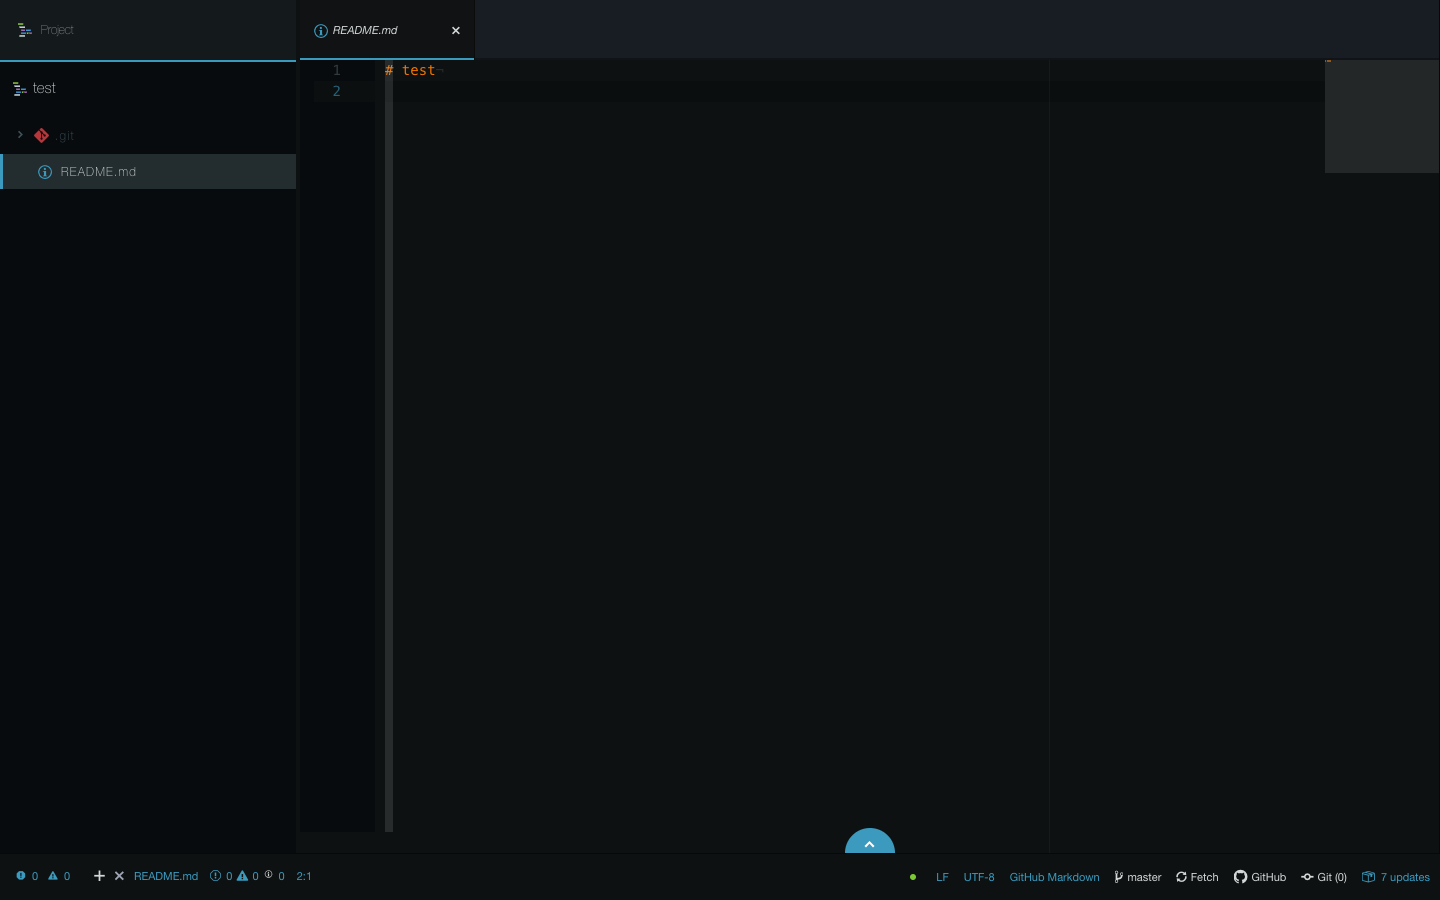
\includegraphics[width=100mm, height=50mm]{../screenshot/github0.png}
        \caption{}
      \end{center}
    \end{figure}
    $\\ \\$

    branchは以下のようにターミナルでコマンドを打つことで作成できる。\\
    また、atom上でもGUIを用いて作成することができる。\\


    \begin{itemize}
      \item branchの確認\\
        $現在作業中のbranchの確認や存在するbranchの確認は以下のコマンドで\\
        \$ \ git \ branch\\
        以下のようにターミナルにコマンドを打つと出力される。\\
        ただし、*がついてるbranchが現在いるbranchである。$

        \begin{figure}[h]
          \begin{center}
            
\includegraphics[width=100mm, height=10mm]{../screenshot/branch0.png}
            \caption{}
          \end{center}
        \end{figure}
        $\\$

        $また、以下のようにatom上の右下にあるmasterのボタンでも簡単に確認できる。\\$
        \begin{figure}[h]
          \begin{center}
            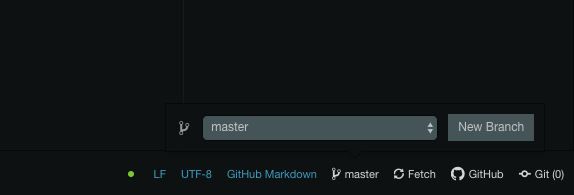
\includegraphics[width=100mm, height=30mm]{../screenshot/branchatom.png}
            \caption{}
          \end{center}
        \end{figure}

      \item branchの作成\\

        $新たにbranchを作る時は以下のようにターミナルでコマンドを打てば作成される。\\
        \$ \ git \ branch \ test\_ branch\\
        以下のようにターミナルにコマンドを打つと出力される。\\$

        \begin{figure}[h]
          \begin{center}
            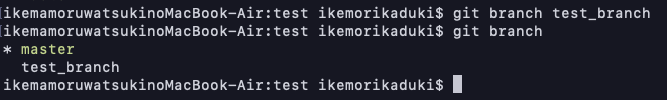
\includegraphics[width=100mm, height=20mm]{../screenshot/makebranch.png}
            \caption{}
          \end{center}
        \end{figure}
        $\\$

        $また、以下のようにatom上の右下にあるmasterのボタンでも簡単に確認できる。\\$
        \begin{figure}[h]
          \begin{center}
            
\includegraphics[width=90mm, height=20mm]{../screenshot/makebranchatom.png}
            \caption{}
          \end{center}
        \end{figure}

      \item branchの切り替え\\
        $新たにbranchを作る時は以下のようにターミナルでコマンドを打てば作成される。\\
        \$ \ git \ checkout \ test\_branch\\
        以下のようにターミナルにコマンドを打つと出力される。$\\

        \begin{figure}[h]
          \begin{center}
            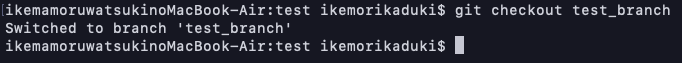
\includegraphics[width=100mm, height=10mm]{../screenshot/gitcheckout.png}
            \caption{}
          \end{center}
        \end{figure}


        $また、以下のようにatom上の右下にあるmasterのボタンでも簡単に切り替えられる。$\\
        \begin{figure}[h]
          \begin{center}
            
\includegraphics[width=120mm, height=20mm]{../screenshot/gitcheckoutatom.png}
            \caption{}
          \end{center}
        \end{figure}
    \end{itemize}
    $\\ \\$

  \subsection{開発用ブランチにcommit}
    $test\_branchでのcommitはいつも通りに、以下のようにすればいい$

    \begin{itemize}
      \item git \ add \ \{追加するファイル名\}
      \item git \ commit \ -m \ \{コミットメッセージ\}
    \end{itemize}
    $また、atom上でも以下の画像のようにcommitを行える。$\\
    $右下のGitボタンを押すと下のように画面が出てくるので、GUIでのaddとcommitが行える。$

    \begin{figure}[ht]
      \begin{center}
        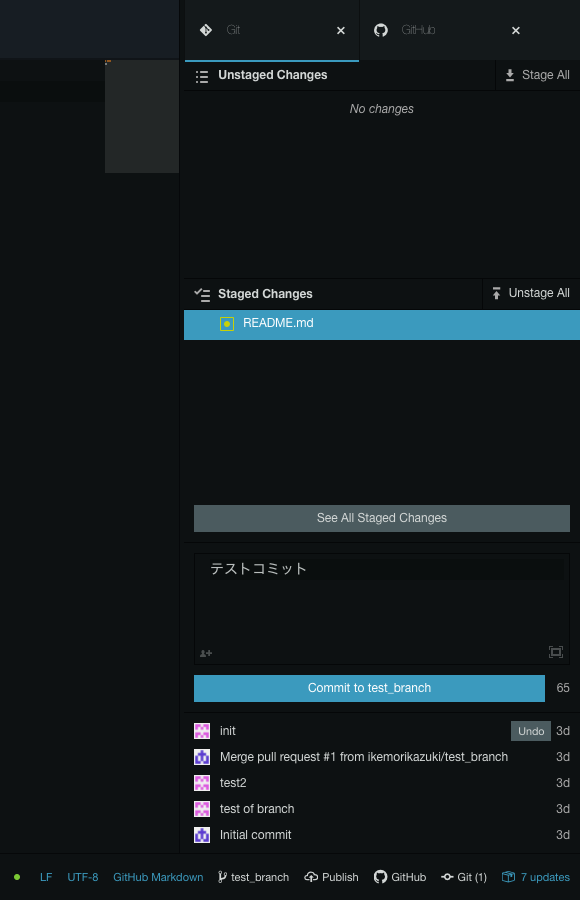
\includegraphics[width=120mm, height=180mm]{../screenshot/addcommitatom.png}
        \caption{}
      \end{center}
    \end{figure}
    $\\ \\$
  \newpage
  \subsection{リモートリポジトリにpushする}
    $test\_branchへのpushは以下のようにterminal上でコマンドを打てばいい。$\\
    $ \$ \ git \ push \ origin \ test\_branch$
    \begin{figure}[ht]
      \begin{center}
        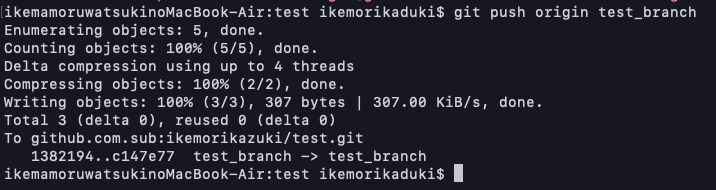
\includegraphics[width=120mm, height=30mm]{../screenshot/push.png}
        \caption{}
      \end{center}
    \end{figure}
    $\\$
    \newpage
    $また、図8の右下にあるpublishボタンを押すことでもpushできる。$

  \subsection{pull requestの送り方}
    github上で以下のような画面になるので、compare \& pull requestを押す。
    \begin{figure}[ht]
      \begin{center}
        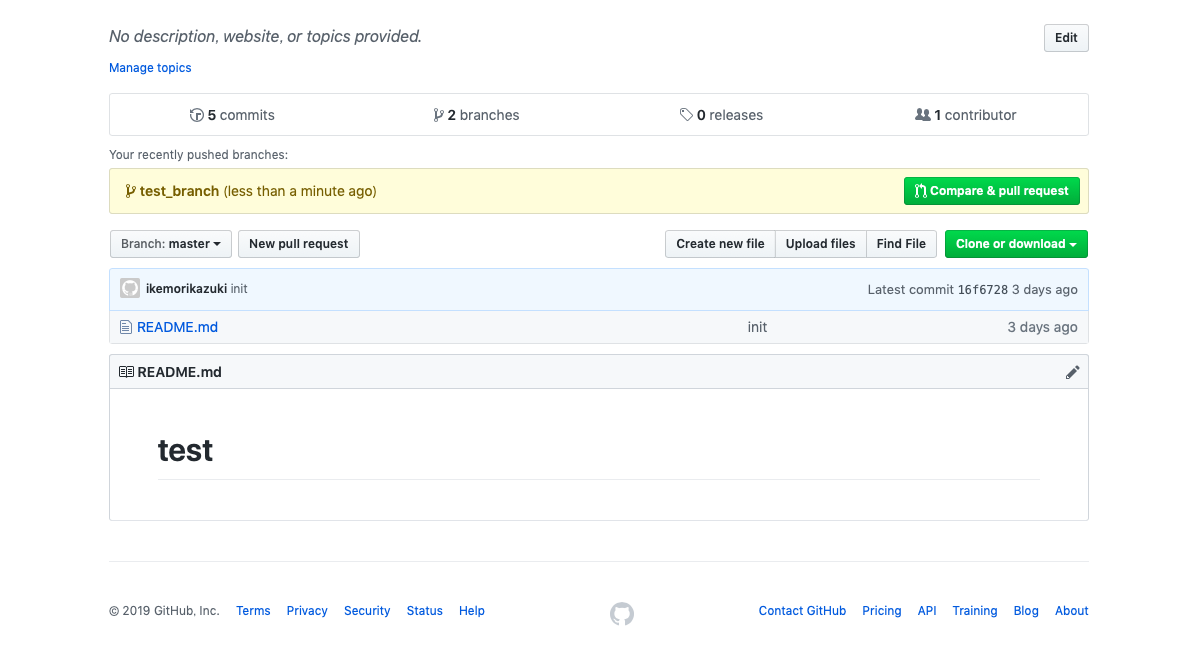
\includegraphics[width=180mm, height=70mm]{../screenshot/pullrequest.png}
        \caption{}
      \end{center}
    \end{figure}

    すると以下のような画面になるので、適当なタイトルとコメントを書いて Create pull requestを押す。
    \begin{figure}[ht]
      \begin{center}
        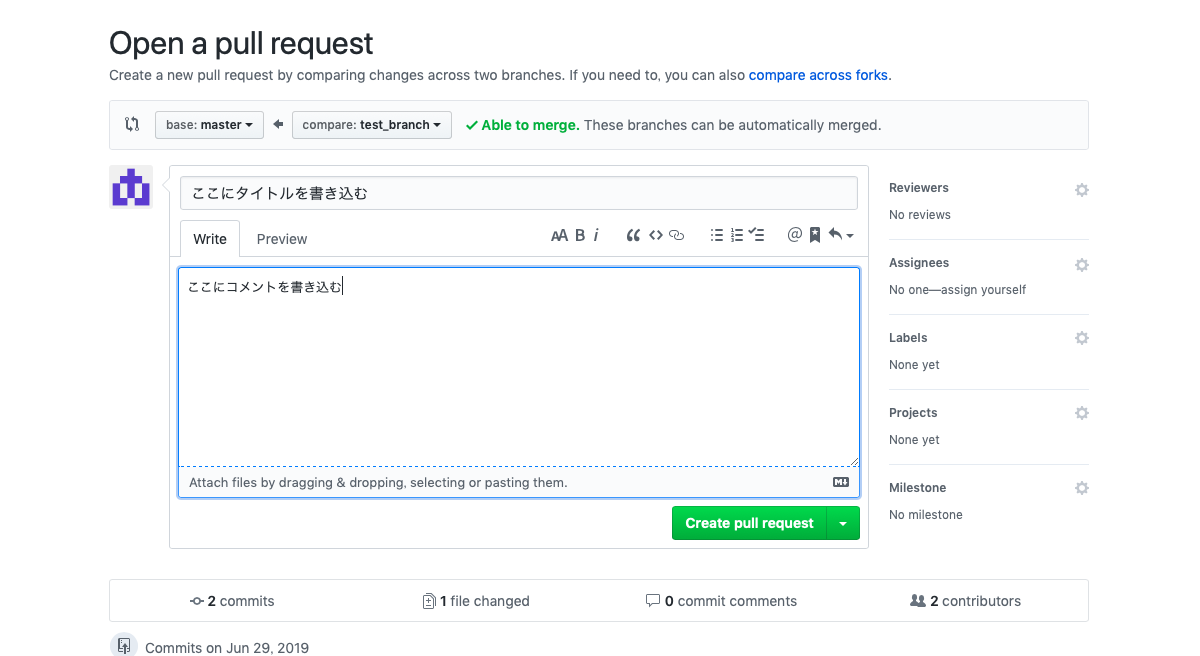
\includegraphics[width=180mm, height=70mm]{../screenshot/pullrequestcoment.png}
        \caption{}
      \end{center}
    \end{figure}
    最後に、問題がなければ以下のような画面になるのでレビュアーのレビューを待ち、訂正を要求されたら訂正する。
    \begin{figure}[ht]
      \begin{center}
        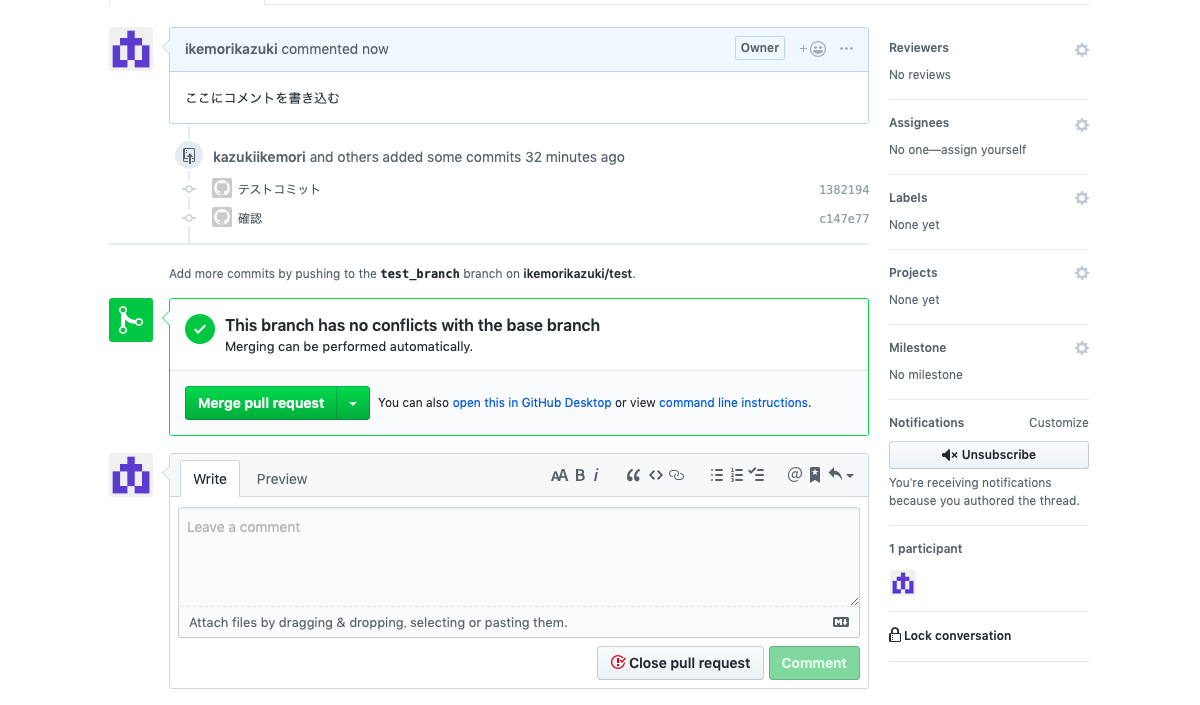
\includegraphics[width=180mm, height=70mm]{../screenshot/merge.png}
        \caption{}
      \end{center}
    \end{figure}

\end{document}
